\input ../SlidePreamble
\input ../preamble

\begin{document}

{\Huge
  
  \centerline{\bf TTIC 31230, Fundamentals of Deep Learning}
  \bigskip
  \centerline{David McAllester, Winter 2019}
  \vfill
  \vfill
  \centerline{\bf Deep Learning Frameworks}
  \vfill
  \vfill

\slideplain{What is a Deep Learning Framework?}

A framework provides a high level language for writing models $P_\Phi(y|x)$.

\vfill
A framework compiles a model into an optimization algorithm.
\vfill
{\color{red} $$\Phi^* \approx \argmin_\Phi E_{(x,y) \sim \mathrm{Train}} \; -\ln P_\Phi(y|x)$$}

\vfill
A framework also typically provides support for managing large training sets and pre-trained model parameter values (also called ``models'').

\slide{Some Frameworks}

\begin{itemize}
  
\item Kaffe

\vfill

\item Tensorflow

\vfill

\item DyNet

  \vfill
\item Chainer

\vfill

\item PyTorch

  \vfill

\item EDF (Educational Framework in Python for this class).
\end{itemize}

$\vdots$

\slide{What Must a Framework Support?}

It must provide a high level language for writing models $P_\Phi(y|x)$ (or other forms of models).

\vfill
It must be able to compile a model into an optimization algorithm.
\vfill
{\color{red} $$\Phi^* \approx \argmin_\Phi E_{(x,y) \sim \mathrm{Train}} \; -\ln P_\Phi(y|x)$$}

\vfill
It typically also provides support for managing large data sets (such as {\color{red} ``$\mathrm{Train}$''} in the above equation).

\slide{An Example: Multi-Layer Perceptron Models for MNIST}

We consider the problem of taking an input $x$ (such as an image of a hand written digit) and classifying it into some small number of classes (such as the digits $0$ through $9$).

\vfill
\centerline{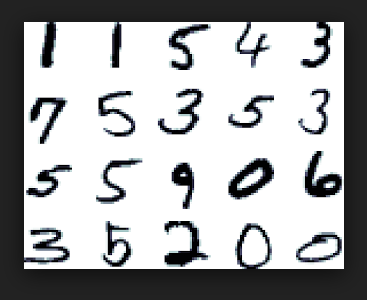
\includegraphics[width= 4.0in]{../images/MNIST}}
  
\slide{Multiclass Classification}

Assume a population distribution on pairs $(x,y)$ for $x \in \reals^d$ and $y \in \{y_1,\ldots, y_k\}$.

\vfill
For MNIST $x$ is a $28 \times 28$ image which we take to be a 784 dimensional vector giving $x \in \reals^{784}$.

\vfill
For MNIST $k = 10$.

\vfill
Let $\mathrm{Train}$ be a sample $(x_0,y_0),\;\ldots,\;(x_{N-1},y_{N-1})$ drawn IID from the population.

\slide{A Multi Layer Perceptron (MLP)}

$$\Phi = (W^0,\;b^0,\;W^1,\;b^1)$$

\begin{eqnarray*}
  {\color{red} h} & = & \sigma\left(W^0{\color{red} x} + b^0\right) \\
  \\
  {\color{red} s} & = & \sigma\left(W^1{\color{red} h} + b^1 \right) \\
  \\
  {\color{red} P_\Phi[\hat{y}]} & = & \softmax_{\hat{y}}\;{\color{red} s[\hat{y}]}
\end{eqnarray*}

\slide{Activation Functions}

An activation function $\sigma:\reals \rightarrow \reals$ (scalar-to-scalar) is applied to each component of a vector.

\vfill
\centerline{{\color{red} $\sigma(u) = \frac{1}{1+e^{-u}}$}\hspace{3em}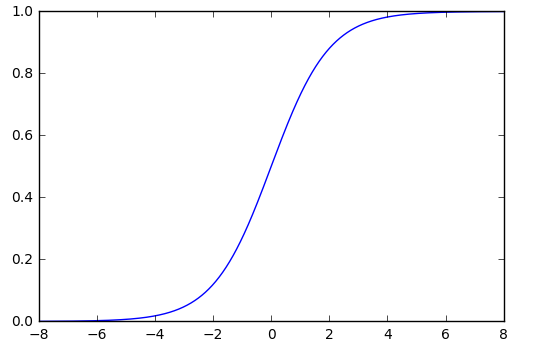
\includegraphics[width=1.5in]{../images/sigmoid}}

\vfill
other common activation functions are

\vfill
\centerline{{\color{red} $\mathrm{ReLU}(u) = \max(0,u)$}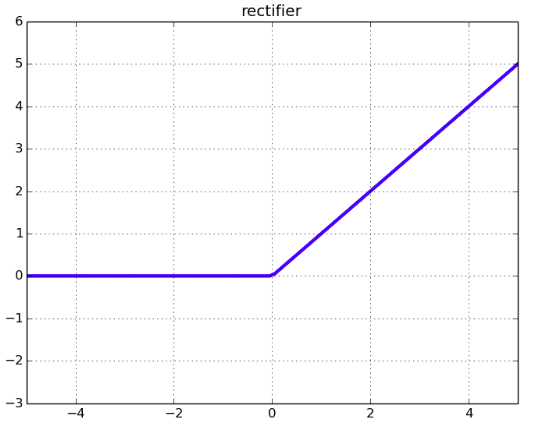
\includegraphics[width=1.5in]{../images/relu},
{\color{red} $\mathrm{tanh}(u) = 2\sigma(u)-1$}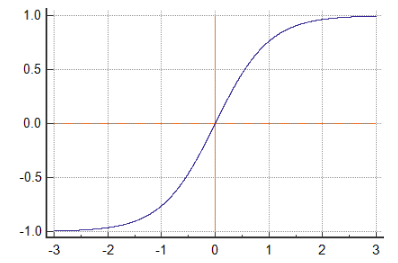
\includegraphics[width=1.5in]{../images/tanh}}

\slide{Optimization}

Once we have specified our model $P_\Phi(y|x)$ in high level equations (such as on the previous two slides) we need to train it.

$$\Phi^* \approx \argmin_\Phi E_{(x,y) \sim {\color{red} \mathrm{Train}}} \; - \ln P_\Phi(y|x)$$

\vfill
The framework generates the training code automatically from the model definition.

\vfill
{\color{red} Optimization is almost always done with some form of stochastic gradient descent (SGD) and the gradient is computed
by back-propagation on the model definition.}

\slide{Stochastic Gradient Descent (SGD)}
$$\Phi^* = \argmin_\Phi E_{(x,y) \sim \mathrm{Train}} \; {\cal L}(x,y,\Phi).$$

\vfill
\begin{enumerate}
\item Randomly Initialize $\Phi$ (initialization is important and must be done with care).

  \vfill
  \item Repeat until ``converged'':

    \vfill
    \begin{itemize}
    \item draw $(x,y) \sim \mathrm{Train}$ at random.
      \vfill
    \item $\Phi \;\;\minuseq\;\; \eta \nabla_\Phi\;{\cal L}(x,y,\Phi)$
    \end{itemize}
\end{enumerate}

\slide{Epochs}

In practice we cycle through the training data visiting each training pair once.

\vfill
One pass through the training data is called an Epoch.

\vfill
One typically imposes a random suffle of the training data before each epoch.

\slide{SGD for MLPs}

$$\Phi = (W^0,\;b^0,\;W^1,\;b^1)$$

\begin{eqnarray*}
  {\color{red} h} & = & \sigma\left(W^0{\color{red} x} + b^0\right) \\
  \\
  {\color{red} s} & = & \sigma\left(W^1{\color{red} h} + b^1 \right) \\
  \\
  {\color{red} P_\Phi[\hat{y}]} & = & \softmax_{\hat{y}}\;{\color{red} s[\hat{y}]}
\end{eqnarray*}

\vfill
We now need to automatically compute $\nabla_\Phi {\cal L}(x,y,\Phi)$.



\ignore{
\slide{Total Gradient Descent}

$${\cal L}_{\mathrm{Train}}(\Phi) = \frac{1}{N}\sum_n {\cal L}(\Phi,x_n,y_n)$$

\vfill
\centerline{We want: \hspace{3ex} $\Phi^*  =  \argmin_\Phi {\cal L}_{\mathrm{Train}}(\Phi)$}

\vfill
$$\Phi \;\;\;\mbox{\tt -=}\;\;\; \eta \nabla_\Phi {\cal L}_\mathrm{Train}(\Phi)$$


\slide{Stochastic Gradient Descent (SGD) on the Training set.}

\vfill
\vfill
repeat:  Select $n$ at random. $\Phi \;\;\minuseq\;\; \eta \;\nabla_\Phi \; {\cal L}(x_n,y_n,\Phi)$

\begin{eqnarray*}
  \expectsub{n}{\nabla_\Phi \; {\cal L}(x_n,y_n,\Phi)} & = & \sum_n P(n) \nabla_\Phi\;{\cal L}_{\mathrm{Train}}(x_n,y_n,\Phi) \\
  \\
  \\ & = & \frac{1}{N} \sum_n \nabla_\Phi\;{\cal L}_{\mathrm{Train}}(x_n,y_n,\Phi) \\
  \\
    \\ & = & \nabla_\Phi \frac{1}{N} \sum_n \;{\cal L}_{\mathrm{Train}}(x_n,y_n,\Phi) \\
  \\
  &  = & \nabla_\Phi\;{\cal L}_{\mathrm{Train}}(\Phi)
\end{eqnarray*}
}

\slideplain{Computation Graphs (Framework Source Code)}

A computation graph (sometimes called a ``computation{\color{red} al} graph'') is a sequence of assignment statements.


\begin{eqnarray*}
  {\color{red} h} & = & \sigma\left(W^0{\color{red} x} + b^0\right) \\
  \\
  {\color{red} s} & = & \sigma\left(W^1{\color{red} h} + b^1 \right) \\
  \\
  {\color{red} P_\Phi[\hat{y}]} & = & \softmax_{\hat{y}}\;{\color{red} s[\hat{y}]}
\end{eqnarray*}

\vfill
I prefer the term ``source code'' to the term ``graph''.

\slideplain{Simpler Source Code}

The expression

\vfill
{\color{red} $${\cal L} = \sqrt{x^2 + y^2}$$}

\vfill
can be transformed to the assignment sequence

{\color{red}
\vfill
\begin{eqnarray*}
  u & = & x^2  \\
  v & = & y^2 \\
  r & =& u + v \\
  {\cal L} & = & \sqrt{r}
\end{eqnarray*}
}

\anaslide{Source Code}
\vspace{-1ex}
{\color{red}
$$\begin{array}{lcl}
 1.\;u & = & x^2  \\
 2.\;w & = & y^2 \\
 3.\;r & =& u + w \\
  4.\;{\cal L} & = & \sqrt{r}
\end{array}$$
}

\vfill
For each variable $z$, the derivative $\partial {\cal L}/\partial z$ will get computed in reverse order.

\vfill
{\color{red}
$$\begin{array}{lcl}
(4)\; \partial{\cal L}/\partial r & = & \frac{1}{2\sqrt{r}} \\
(3)\; \partial{\cal L}/\partial u & = & \partial {\cal L}/\partial r \\
(3)\; \partial{\cal L}/\partial w & = & \partial {\cal L}/\partial r\\
(2)\; \partial{\cal L}/\partial y & = & (\partial {\cal L}/\partial w) * (2y) \\
(1)\; \partial{\cal L}/\partial x & = & (\partial {\cal L}/\partial u) * (2x)
\end{array}$$
}

\anaslideplain{A More Abstract Example (Still Scalar Values)}
\vspace{-3ex}
\begin{eqnarray*}
  y & = & f(x) \\
  z & = & g(y,x) \\
  u & = & h(z) \\
  {\cal L} & = & u
\end{eqnarray*}

\medskip
For now assume all values are scalars.

\medskip
We will ``backpopagate'' the assignments the reverse order.

\anaslide{Backpropagation (Scalar Values)}
\vspace{-3ex}
\begin{eqnarray*}
  y & = & f(x) \\
  z & = & g(y,x) \\
  u & = & h(z) \\
  {\cal L} &  = & {\color{red} u}
\end{eqnarray*}

\medskip
{\color{red} ${\partial {\cal L}}/{\partial u} = 1$}

\anaslide{Backpropagation (Scalar Values)}
\vspace{-3ex}
\begin{eqnarray*}
  y & = & f(x) \\
  z & = & g(y,x) \\
  u & = & h({\color{red} z}) \\
  {\cal L} &  = &  u
\end{eqnarray*}

\medskip
${\partial {\cal L}}/{\partial u} = 1$

\medskip
{\color{red} ${\partial {\cal L}}/{\partial z} = ({\partial {\cal L}}/{\partial u})\; ({\partial h}/{\partial z})$} (this uses the value of $z$)

\anaslide{Backpropagation (Scalar Values)}
\vspace{-3ex}
\begin{eqnarray*}
  y & = & f(x) \\
  z & = & g({\color{red} y},x) \\
  u & = & h(z) \\
  {\cal L} &  = &  u
\end{eqnarray*}

\medskip
${\partial {\cal L}}/{\partial u} = 1$

\medskip
${\partial {\cal L}}/{\partial z} = ({\partial {\cal L}}/{\partial u})\; ({\partial h}/{\partial z})$

\medskip
{\color{red} ${\partial {\cal L}}/{\partial y} = ({\partial {\cal L}}/{\partial z})\; ({\partial g}/{\partial y})$} (this uses the value of $y$ and $x$)

\anaslide{Backpropagation (Scalar Values)}
\vspace{-3ex}
\begin{eqnarray*}
  y & = & f({\color{red} x}) \\
  z & = & g(y,{\color{red} x}) \\
  u & = & h(z) \\
  {\cal L} &  = &  u
\end{eqnarray*}

\medskip
${\partial {\cal L}}/{\partial u} = 1$

\medskip
${\partial {\cal L}}/{\partial z} = ({\partial {\cal L}}/{\partial u})\; ({\partial h}/{\partial z})$

\medskip
${\partial {\cal L}}/{\partial y} = ({\partial {\cal L}}/{\partial z})\; ({\partial g}/{\partial y})$

\medskip
{\color{red} ${\partial {\cal L}}/{\partial x} =$ ???} Oops, we need to add up multiple occurrences.

\anaslide{Backpropagation (Scalar Values)}
\vspace{-3ex}
\begin{eqnarray*}
  y & = & f({\color{red} x}) \\
  z & = & g(y,{\color{red} x}) \\
  u & = & h(z) \\
  {\cal L} &  = &  u
\end{eqnarray*}

\medskip
Each framework program variable denotes an {\color{red} object} (in the sense of C++ or Python).

\medskip
{\color{red} $x.\mathrm{value}$} and {\color{red} $x.\grad$} are attributes of the {\color{red} object $x$}.

\bigskip
Values are computed ``forward'' while gradients are computed ``backward''.


\anaslide{Backpropagation (Scalar Values)}
\vspace{-3ex}
\begin{eqnarray*}
  y & = & f(x) \\
  z & = & g(y,x) \\
  u & = & h(z) \\
  {\color{red} {\cal L}} &  {\color{red} =} & {\color{red}  u}
\end{eqnarray*}


\bigskip
We initialize {\color{red} $x.\mathrm{grad}$} to zero: {\color{red} $z.\grad = y.\grad = x.\grad = 0$}

\bigskip
We initialize the loss gradient to 1: {\color{red} $u.\grad = 1$}

\medskip
{\bf Loop Invariant}: For any variable $w$ whose definition has not yet been processed we have that $w.\grad$ is $\partial {\cal L}/\partial w$ as defined by the set of assignments already processed.

\anaslide{Backpropagation (Scalar Values)}
\vspace{-3ex}
\begin{eqnarray*}
  y & = & f(x) \\
  z & = & g(y,x) \\
  {\color{red} u} & {\color{red} =} & {\color{red} h(z)} \\
  {\color{red} {\cal L}} & {\color{red}  =} &  {\color{red} u}
\end{eqnarray*}

{\color{red}
\medskip
$z.\grad = y.\grad = x.\grad = 0$

\medskip
$u.\grad = 1$

\medskip
$z.\grad\;\pluseq\; u.\grad * {\partial h}/{\partial z}$

}

\medskip
{\bf Loop Invariant}: For any variable $w$ whose definition has not yet been processed we have that $w.\grad$ is $\partial {\cal L}/\partial w$ as defined by the set of assignments already processed.

\anaslide{Backpropagation (Scalar Values)}
\vspace{-3ex}
\begin{eqnarray*}
  y & = & f(x) \\
  {\color{red} z} & {\color{red} =} & {\color{red} g(y,x)} \\
  {\color{red} u} & {\color{red} =} & {\color{red} h(z)} \\
  {\color{red} {\cal L}} & {\color{red} =} & {\color{red}  u}
\end{eqnarray*}

{\color{red}
\medskip
$z.\grad = y.\grad = x.\grad = 0$

\medskip
$u.\grad = 1$

\medskip
$z.\grad\;\pluseq\; u.\grad * {\partial h}/{\partial z}$

\medskip
$y.\grad \;\pluseq\; z.\grad * {\partial g}/{\partial y}$

\medskip
$x.\grad \;\pluseq\; z.\grad * {\partial g}/{\partial x}$

}

\medskip
    {\bf Loop Invariant}: For any variable $w$ whose definition has not yet been processed we have that $w.\grad$ is $\partial {\cal L}/\partial w$ as defined by the set of assignments already processed.

\anaslideplain{Backpropagation (Scalar Values)}
\vspace{-3ex}
\begin{eqnarray*}
  {\color{red} y} & {\color{red} =} & {\color{red} f(x)} \\
  {\color{red} z} & {\color{red} =} & {\color{red} g(y,x)} \\
  {\color{red} u} & {\color{red} =} & {\color{red} h(z)} \\
  {\color{red} {\cal L}} & {\color{red} =} & {\color{red} u}
\end{eqnarray*}

{\color{red}
\medskip
$z.\grad = y.\grad = x.\grad = 0$

\medskip
$u.\grad = 1$

\medskip
$z.\grad\;\pluseq\; u.\grad * {\partial h}/{\partial z}$

\medskip
$y.\grad \;\pluseq\; z.\grad * {\partial g}/{\partial y}$

\medskip
$x.\grad \;\pluseq\; z.\grad * {\partial g}/{\partial x}$

\medskip
$x.\grad \;\pluseq\; y.\grad * {\partial f}/{\partial x}$
}

\ignore{
\anaslide{The Vector-Valued Case}
\vspace{-3ex}
\begin{eqnarray*}
  y & = & f(x) \\
  z & = & g(y,x) \\
  u & = & h(z) \\
  {\cal L} & = & u
\end{eqnarray*}

\vfill
Now suppose the variables can be  vector-valued.

\vfill
The loss ${\cal L}$ is still a scalar.

\vfill
In this case
$$x.\mathrm{grad} = \nabla_x\;{\cal L}$$
}

\slide{Handling Vectors, Arrays, and Tensors}


\begin{eqnarray*}
  {\color{red} h} & = & \sigma\left(W^0{\color{red} x} + b^0\right) \\
  \\
  {\color{red} s} & = & \sigma\left(W^1{\color{red} h} + b^1 \right) \\
  \\
  {\color{red} P_\Phi[\hat{y}]} & = & \softmax_{\hat{y}}\;{\color{red} s[\hat{y}]}
\end{eqnarray*}

\vfill
Each array (tensor) {\color{red} $W$} is an object with attributes {\color{red} $W.\mathrm{value}$} and a gradient {\color{red} $W.\mathrm{grad}$}.

\vfill
The attribute {\color{red} $W.\mathrm{grad}$} is an array (tensor) with the same indeces as {\color{red} $W.\mathrm{value}$}.

\slide{Einstein Notation}

\centerline{$i$ --- input feature index \hspace{1em} $j$  --- hidden layer index, \hspace{1em} $\hat{y}$ --- possible label}
$$\Phi = (W^0[j,i],\;b^0[j],\;W^1[\hat{y},j],\;b^1[\hat{y}])$$

\vfill
\begin{eqnarray*}
  {\color{red} h[j]} & = & \sigma\left(\left(\sum_i\;W^0[j,i] \;{\color{red} x[i]}\right) + b^0[j]\right) \\
  \\
  {\color{red} s[\hat{y}]} & = & \sigma\left(\left(\sum_j\;W^1[\hat{y},j]\;{\color{red} h[j]}\right) + b^1[\hat{y}]\right) \\
  \\
  {\color{red} P_\Phi[\hat{y}]} & = & \softmax_{\hat{y}}\;{\color{red} s[\hat{y}]}
\end{eqnarray*}

\slide{The Swap Rule}
\vspace{-3ex}
\begin{eqnarray*}
  \tilde{y}[j] & = & \sum_i\;W[j,i]\;x[i] \\
  \\
  y[j] & = & \sigma(\tilde{y}[j] + b[j]) \\
  \end{eqnarray*}

\vspace{-5ex}
{\color{red} 
  \begin{eqnarray*}
  \\
  x.\mathrm{grad}[i] & \pluseq & \sum_j\;\tilde{y}.\mathrm{grad}[j]W[j,i] \\
  \\
  W.\mathrm{grad}[j,i] & \pluseq & \tilde{y}.\mathrm{grad}[j]x[i]
\end{eqnarray*}
}

one swaps the output with one of the inputs and sums over the indeces not occuring on the left.

\slideplain{Minibatching}

Training time is greatly improved by minibatching.

 \vfill
{\bf Minibatching}: We run some number of instances together (or in parallel) and then do a parameter update based on the average
gradients of the instances of the batch.

\vfill
For NumPy minibatching is not so much about parallelism as about making the vector operations larger so that the vector operations dominate
the slowness of Python.  On a GPU minibatching allows parallelism over the batch elements.
\vfill

\slide{Minibatching}
\vfill
With minibatching each input value and each computed value is actually a batch of values.

\vfill
We add a batch index as an additional first tensor dimension for each input and computed node.

\vfill
Parameters do not have a batch index.

\slide{Einstein Notation with Minibatching}

\centerline{$b$--- batch index,\hspace{3em} $i$ --- input feature index}
\centerline{$j$ --- hidden layer index, \hspace{3em} $\hat{y}$ --- possible label}
$$\Phi = (W^0[j,i],\;b^0[j],\;W^1[\hat{y},j],\;b^1[\hat{y}])$$

\vfill
\begin{eqnarray*}
  {\color{red} h[b,j]} & = & \sigma\left(\left(\sum_i\;W^0[j,i] \;{\color{red} x[b,i]}\right) + b^0[j]\right) \\
  \\
  {\color{red} s[b,\hat{y}]} & = & \sigma\left(\left(\sum_j\;W^1[\hat{y},j]\;{\color{red} h[b,j]}\right) + b^1[\hat{y}]\right) \\
  \\
  {\color{red} P_\Phi[b,\hat{y}]} & = & \softmax_{\hat{y}}\;{\color{red} s[b,\hat{y}]}
\end{eqnarray*}

\slideplain{The Swap Rule with Minibatching}
\vspace{-3ex}
\begin{eqnarray*}
\vdots \\
  \tilde{y}[b,j] & = & \sum_i\;W[j,i]\;x[b,i] \\
  \vdots
  \end{eqnarray*}

  \begin{eqnarray*}
  \\
  x.\mathrm{grad}[b,i] & \pluseq & \sum_j\;\tilde{y}.\mathrm{grad}[b,j]W[j,i] \\
  \\
  W.\mathrm{grad}[j,i] & \pluseq & {\color{red} \frac{1}{B} \sum_b}\;\tilde{y}.\mathrm{grad}[b,j]x[b,i]
\end{eqnarray*}

\slide{Summary}

A framework provides a high level language for writing models $P_\Phi(y|x)$.

\vfill
A framework compiles a model into an optimization algorithm.
\vfill
{\color{red} $$\Phi^* \approx \argmin_\Phi E_{(x,y) \sim \mathrm{Train}} \; -\ln P_\Phi(y|x)$$}

\vfill
A framework also typically provides support for managing large training sets and pre-trained model parameter values (also called ``models'').

 
\slide{END}
}
\end{document}
